\documentclass[10pt]{beamer}

% NOTE %
% In order to compile this file as is, you'll need a few things:
%   1. mtheme (https://github.com/matze/mtheme)
%   2. Fira Sans font from Mozilla (https://www.mozilla.org/en-US/styleguide/products/firefox-os/typeface/)
% In addition, you'll need to compile using XeTeX.  If that all sounds too complicated, just change the theme below.

\usetheme{m}

\usepackage{spot}
\usepackage{color}
\usepackage{booktabs}
\usepackage{makecell}

\title{Setting the Stage}
\subtitle{}

\author{{\large Dana C.~Ernst}\\
Northern Arizona University}
\date{}

\begin{document}

\setspotlightstyle{rectangle, rounded corners,fill=structure.fg!15!white,path fading=none}

\maketitle

%% ----------------------------------------------------------------------

\section{Activity 1}

%% ----------------------------------------------------------------------  

\begin{frame}{Directions}

\vspace{3em}

\begin{block}{Directions}
\vspace{-.5em}
\begin{itemize}
\item Get in groups of size 3--4.
\item Group members should introduce themselves.
\item For each of the questions that follow, I will ask you to:
\begin{enumerate}
\item \alert{Think} about a possible answer on your own.
\item \alert{Discuss} your answers with the rest of your group.
\item \alert{Share} a summary of each group's discussion.
\end{enumerate}
\end{itemize}
\end{block}

\end{frame}

%% ----------------------------------------------------------------------

\section{Questions}

%% ----------------------------------------------------------------------

\begin{frame}%{Question One}
\ 

\vfill

\spot[inner sep=2ex]{{
\parbox{\linewidth}{
\Large What are the goals of a university education?}
}}

\vfill

\end{frame}

%% ----------------------------------------------------------------------

\begin{frame}%{Question Two}
\ 

\vfill

\spot[inner sep=2ex]{{
\parbox{\linewidth}{
\Large How does a person learn something new?}
}}

\vfill

\end{frame}

%% ----------------------------------------------------------------------

\begin{frame}%{Question Three}
\ 

\vfill

\spot[inner sep=2ex]{{
\parbox{\linewidth}{
\Large What do you reasonably expect to remember from your courses in 20 years?}
}}

\vfill

\end{frame}

%% ----------------------------------------------------------------------

\begin{frame}%{Question Four}
\ 

\vfill

\spot[inner sep=2ex]{{
\parbox{\linewidth}{
\Large What is the value of making mistakes in the learning process?}
}}

\vfill

\end{frame}

%% ----------------------------------------------------------------------

%\begin{frame}{Question Five}
%\ 
%
%\spot[inner sep=2ex]{{
%\parbox{\linewidth}{
%\Large How do we create a safe environment where risk taking is encouraged and productive failure is valued?}
%}}
%
%\end{frame}

%% ----------------------------------------------------------------------

\section{Activity 2}

%% ----------------------------------------------------------------------  

\begin{frame}{Deep Practice}

\vspace{2em}

Take 45 seconds to look over the following list of pairs of words, but do not write anything down.

\begin{table}[h]
\centering
\begin{tabular}{@{}ll@{}}
\toprule
bread/b\underline{\ \ }tter & ocean/breeze \\
leaf/tree & music/l\underline{\ \ }rics\\
sweet/sour & sh\underline{\ \ }e/sock\\
phone/bo\underline{\ \ }k & movie/actress \\
chi\underline{\ \ }s/salsa & gasoline/engine \\
high school/college & pen\underline{\ \ }il/paper\\
river/b\underline{\ \ }at & turkey/stuffing \\
fruit/vegetable & be\underline{\ \ }r/wine\\
computer/chip & television/rad\underline{\ \ }o\\
l\underline{\ \ }nch/dinner & chair/couch \\
\bottomrule
\end{tabular}
\end{table}

\end{frame}

%% ----------------------------------------------------------------------  

\begin{frame}{Deep Practice}

\vspace{2em}

\begin{block}{Directions}
\vspace{-.75em}
\begin{itemize}
\item Without looking at the list of pairs of words, write down as many pairs as you can.  You do not need to remember where any missing letters were nor which column a pair was in.
\item Looking at the table on the next slide count how many pairs are in column A versus column B.
\end{itemize}
\end{block}

\end{frame}

%% ----------------------------------------------------------------------  

\begin{frame}{Deep Practice}

\vspace{2em}

\begin{table}[h]
\centering
\begin{tabular}{@{}ll@{}}
\toprule
\makecell[c]{A} & \makecell[c]{B}  \\
\midrule
ocean/breeze & bread/b\underline{\ \ }tter\\
leaf/tree & music/l\underline{\ \ }rics\\
sweet/sour & sh\underline{\ \ }e/sock\\
movie/actress & phone/bo\underline{\ \ }k\\
gasoline/engine & chi\underline{\ \ }s/salsa\\
high school/college & pen\underline{\ \ }il/paper\\
turkey/stuffing & river/b\underline{\ \ }at\\
fruit/vegetable & be\underline{\ \ }r/wine\\
computer/chip & television/rad\underline{\ \ }o\\
chair/couch & l\underline{\ \ }nch/dinner\\
\bottomrule
\end{tabular}
\caption{Word list from \alert{The Talent Code}.}
\end{table}

\end{frame}

%% ----------------------------------------------------------------------  

\begin{frame}{Deep Practice}

\vspace{2em}

According to \alert{The Talent Code} by Daniel Coyle, studies show that on average people remember 3 times as many pairs in column B, the one with missing letters. Maybe a room full of mathematicians will have wildly different results\ldots 

\vspace{1em}

\onslide<2->{The claim is that a microsecond of struggle (cognitive demand) makes all the difference.}

\end{frame}

%% ----------------------------------------------------------------------

\section{Discussion}

%% ----------------------------------------------------------------------

\begin{frame}{The Big Picture}

\vspace{2em}

\begin{block}{Claims}
\vspace{-.75em}
\begin{itemize}
\item An education must prepare a student to ask and explore questions in contexts that do not yet exist. That is, we need individuals capable of tackling problems they have never encountered and to ask questions no one has yet thought of.
\item If we really want students to be independent, inquisitive, \& persistent, then we need to provide them with the means to acquire these skills.
\end{itemize}
\end{block}

\pause

\begin{block}{Some items to be aware of}
\vspace{-.75em}
\begin{itemize}
\item This class requires \alert{active learning} and \alert{mindful preparation}. 
%\item Our experience in the course is based directly on the things you pointed out as being important: \alert{active and independent learning}, \alert{productive failure}, and \alert{working in a community}.  
\item My role in the course is \alert{consultant}, \alert{instructional designer}, \alert{feedback-giver}, \alert{mentor in the middle}. 
\end{itemize}
\end{block}

%\begin{block}{Lofty Goals}
%\vspace{-.75em}
%\begin{itemize}
%\item Transition students from consumers to producers!
%\item I want to provide the opportunity for a transformative experience. 
%\item I want to change my students' lives!
%\end{itemize}
%\end{block}

\end{frame}

%% ----------------------------------------------------------------------

\begin{frame}{Productive Failure \& Productive Struggle}

\vspace{3em}

\spot[inner sep=2ex]{{
\parbox{\linewidth}{
\Large \alert{``Any creative endeavor is built on the ash heap of failure."} --- Michael Starbird}
}}

\vspace{3em}

\spot[inner sep=2ex]{{
\parbox{\linewidth}{
\Large \alert{``You will become clever through your mistakes."} — German Proverb}
}}

\vspace{3em}

\spot[inner sep=2ex]{{
\parbox{\linewidth}{
\Large \alert{``If you want to sharpen a sword, you have to remove a little metal."} --- Unknown}
}}

\end{frame}

%% ----------------------------------------------------------------------  

\begin{frame}{Stepping Stones}

\vspace{1em}

\begin{center}
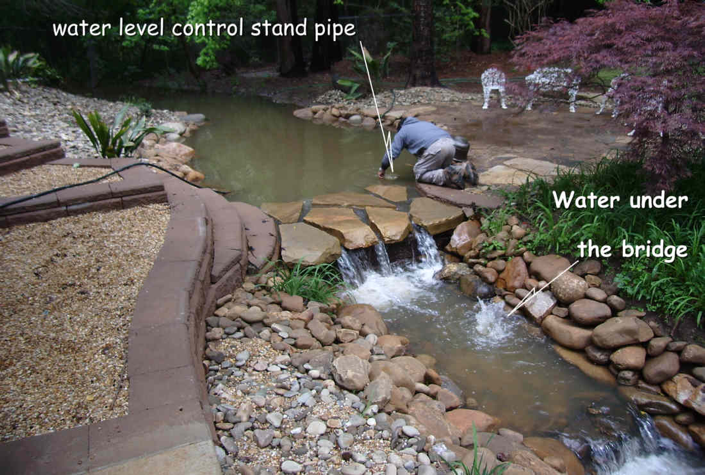
\includegraphics[height=1.4in]{Rocks1} \hspace{.1cm} 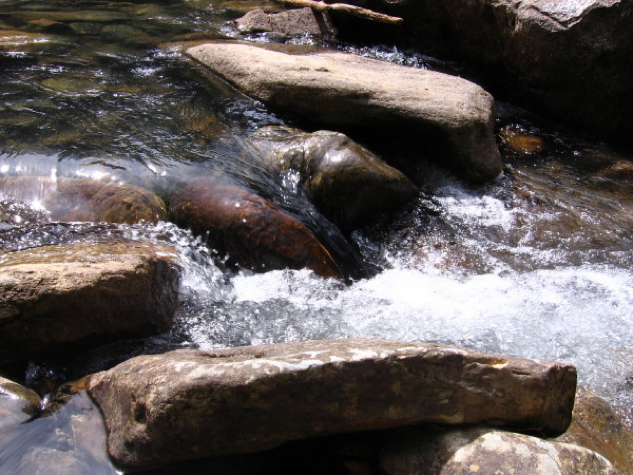
\includegraphics[height=1.4in]{Rocks2}

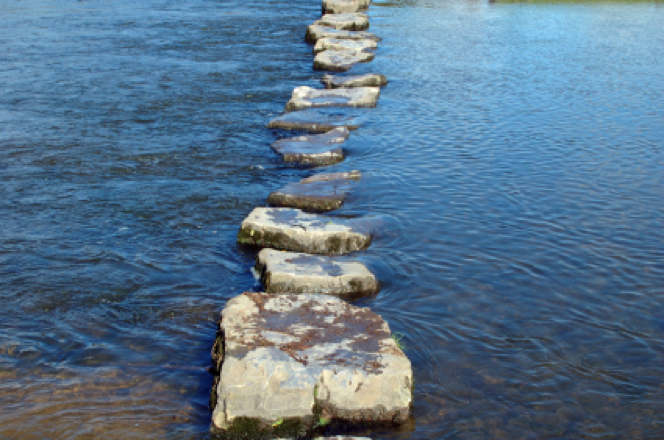
\includegraphics[height=1.4in]{Rocks3}
\end{center}

\vspace{-1em}

{\small \emph{Note:} Analogy inspired by Patrick Rault (University of Arizona).}

\end{frame}

%% ----------------------------------------------------------------------

%\begin{frame}{One Final Quote}
%
%\ 
%\ 
%\ 
%
%\vfill
%
%\spot[inner sep=2ex]{{
%\parbox{\linewidth}{
%\Large \alert{``Every time that a human being succeeds in making an effort of attention with the sole idea of increasing his grasp of truth, he acquires a greater aptitude for grasping it, even if his effort produces no visible fruit."} --- Simone Weil}
%}}
%
%\vfill
%
%\end{frame}

%% ----------------------------------------------------------------------

\end{document}
